\chapter{Methods}
\label{ch:methods}
We have decided on the following approach for the autonomous avoidance system. We use four different ToF ranging sensors each mounted on one side and pointing in either negative or positive x-direction, or in either negative or positive y-direction (\cref{fig:sketch}). The sensors sends the data to the \textit{mbed LPC1768} microcontroller from which the ranging data is send forward to the \textit{pixhawk} autopilot. The pixhawk uses the ranging data to compute the repulsive force pushing the platform away from the obstacle. The repulsive force is derived from an artificial potential field which exponentially increases towards an obstacle. The force is converted into corrective attitude angles and send to the low-level attitude controller, where the corrective angles are added to the attitude set-point. The controller then computes the required thrust for each motor (\cref{fig:approach}). Eventually, the drone should repel itself from the obstacle.\\
For a successful implementation of a potential field we have decided on the following methodology:
\begin{enumerate}
	\item Evaluation of the \textit{VL53L0X} ToF Ranging Sensor with a \textit{mbed LPC1768} microcontroller on its potential use for obstacle avoidance on a MAV (\cref{sec:ranging sensor})
	\item Integration of four \textit{VL53L0X} sensors in the pixhawk autopilot (\cref{sec:pixhawk}).
	\item Implementation of a potential field on the pixhawk (\cref{sec:potential field}).
	\item Testing the whole system.  (\cref{sec:testing})
\end{enumerate}
\begin{figure}
	\centering
	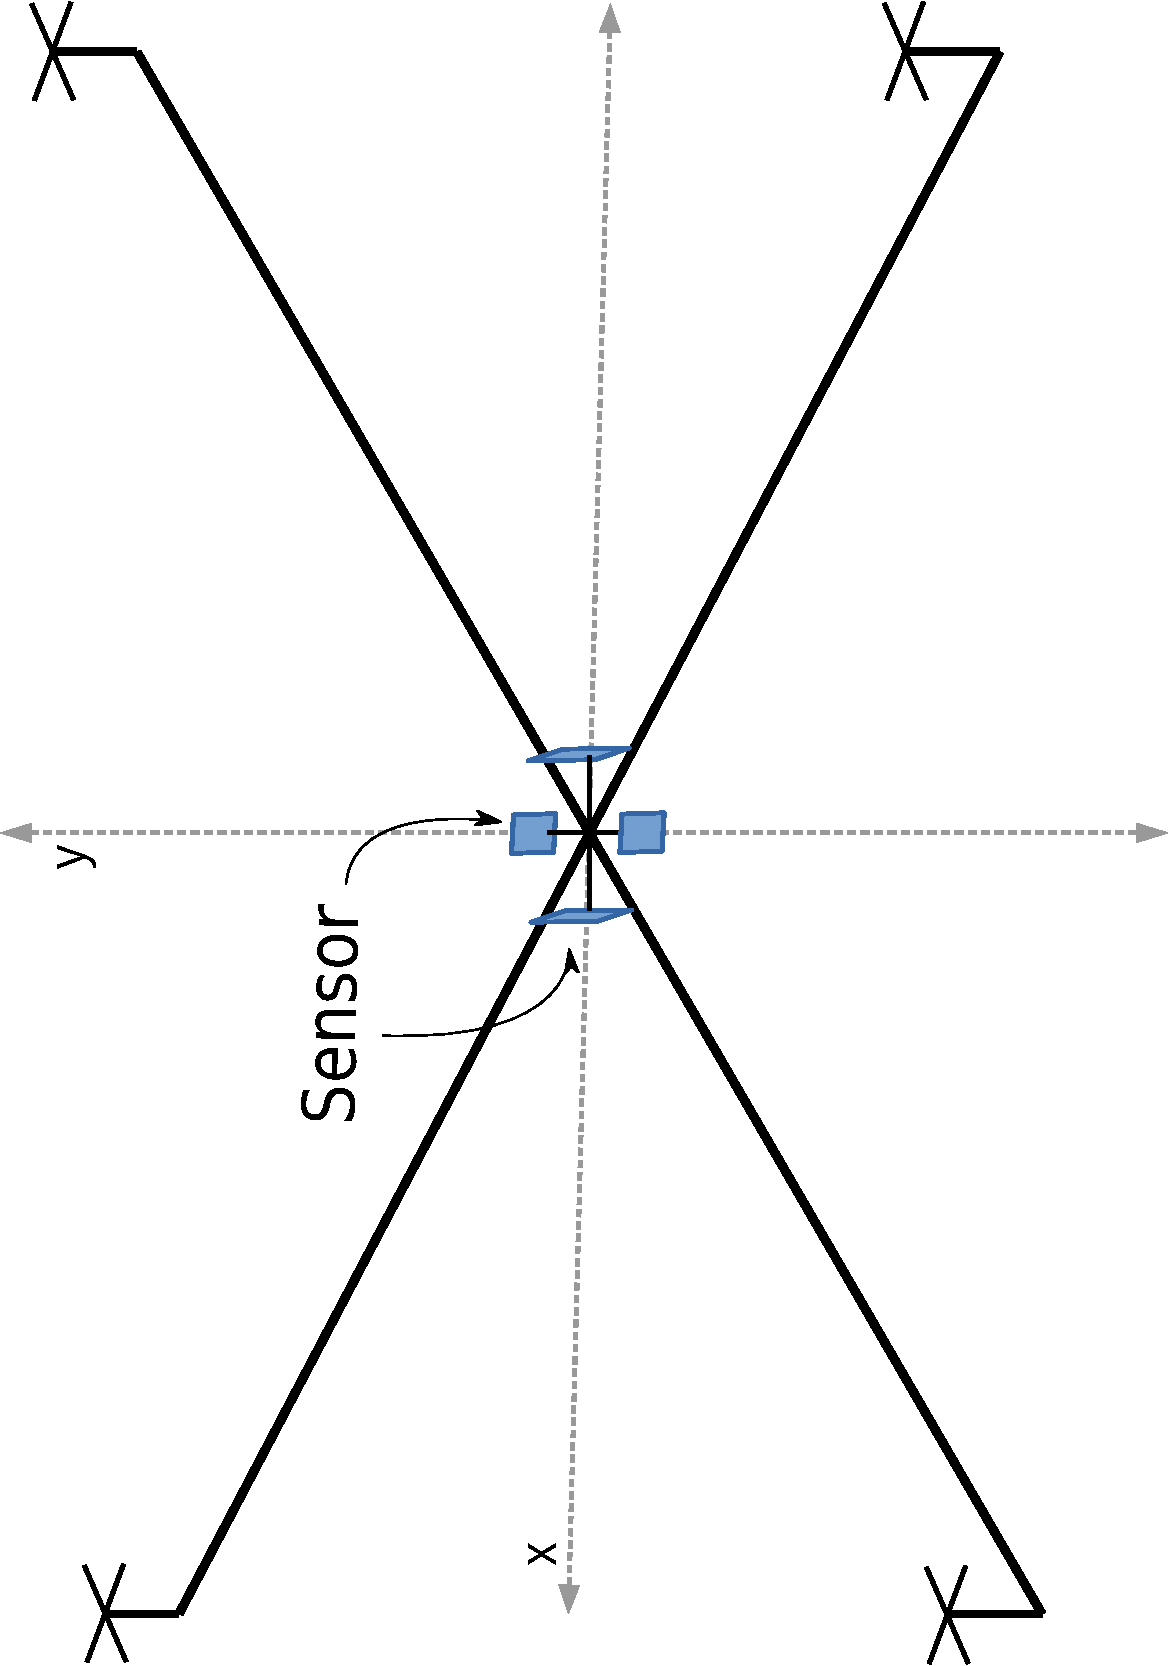
\includegraphics[width=0.4\linewidth, angle = 270]{pictures/mav_sketch.pdf}
	\caption{Sketch of the sensor's setup on the MAV.}
	\label{fig:sketch}
\end{figure}

\begin{figure}
	\centering
	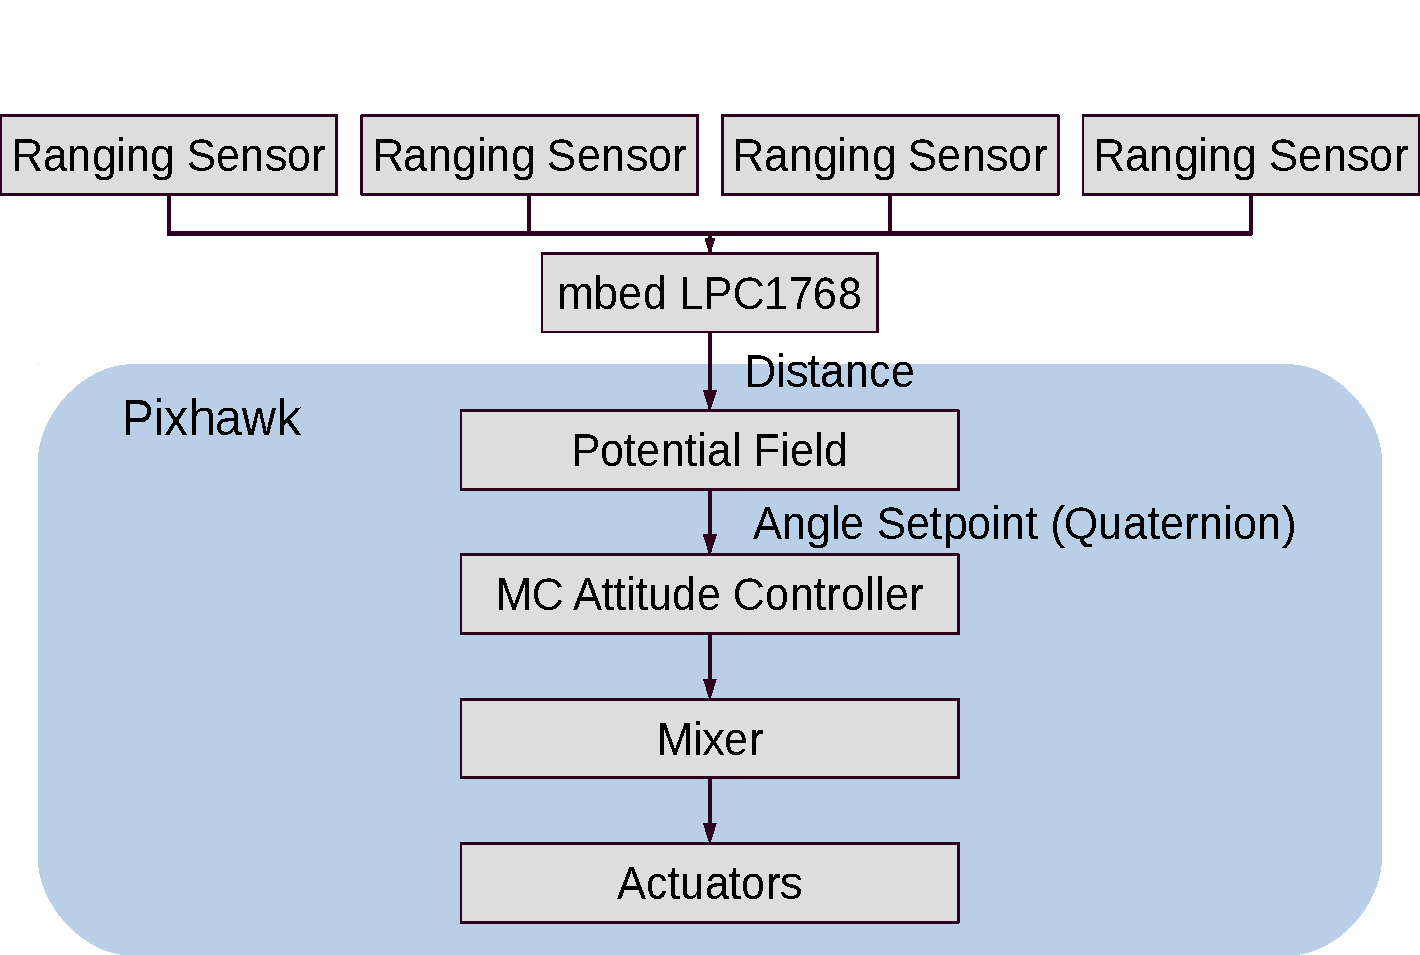
\includegraphics[width=0.8\linewidth]{pictures/approach.pdf}
	\caption{Approach for obstacle avoidance.}
	\label{fig:approach}
\end{figure}
\section{Ranging Sensor}
\label{sec:ranging sensor}
Major constraint for MAVs are payload and available power, thus, we need a low power and on the same time lightweight ranging sensor for our avoidance system. We've opted for the \textit{VL53L0X} ToF Ranging Sensor developed by \textit{STMicroelectronics} (\cref{fig:sensor}) for the distance measurements. For the evaluation we connected the sensor via I2C bus to a \textit{mbed LPC1768} microcontroller. The sensor has a range of \unit[0]{mm} up to \unit[2]{m} at optimal conditions, i.e., no infrared radiation (IR). With a IR source the sensor has a range of \unit[0]{m} to \unit[1.2]{m}.  The sensor allows four different modes to be used (\cref{tab:profile}). To facilitate the integration we use the \textit{53L0-SATEL-I1} satellite board (\cref{fig:satellite}) \cite{boardVL53L0X}. As defined by the manufacturer, the satellite board can be used with a power supply ranging from \unit[2.8]{V} up to \unit[5]{V}. The PCB section supporting the VL53L0X module is perforated so that developers can break off the mini PCB for use in a 2.8V supply application. The PCB can be utilized for further miniaturisation. The VL53L0X sensor comes with a Application Programming Interface (API) which allows to control the VL53L0X firmware like initialisation/calibration, ranging Start/Stop, choice of accuracy and choice of ranging mode. If the sensor is not able to make a measurement or the target is outside of its range, the API returns a value greater than 8000 \cite{VL53L0X}.\\
\begin{figure}
	\centering
	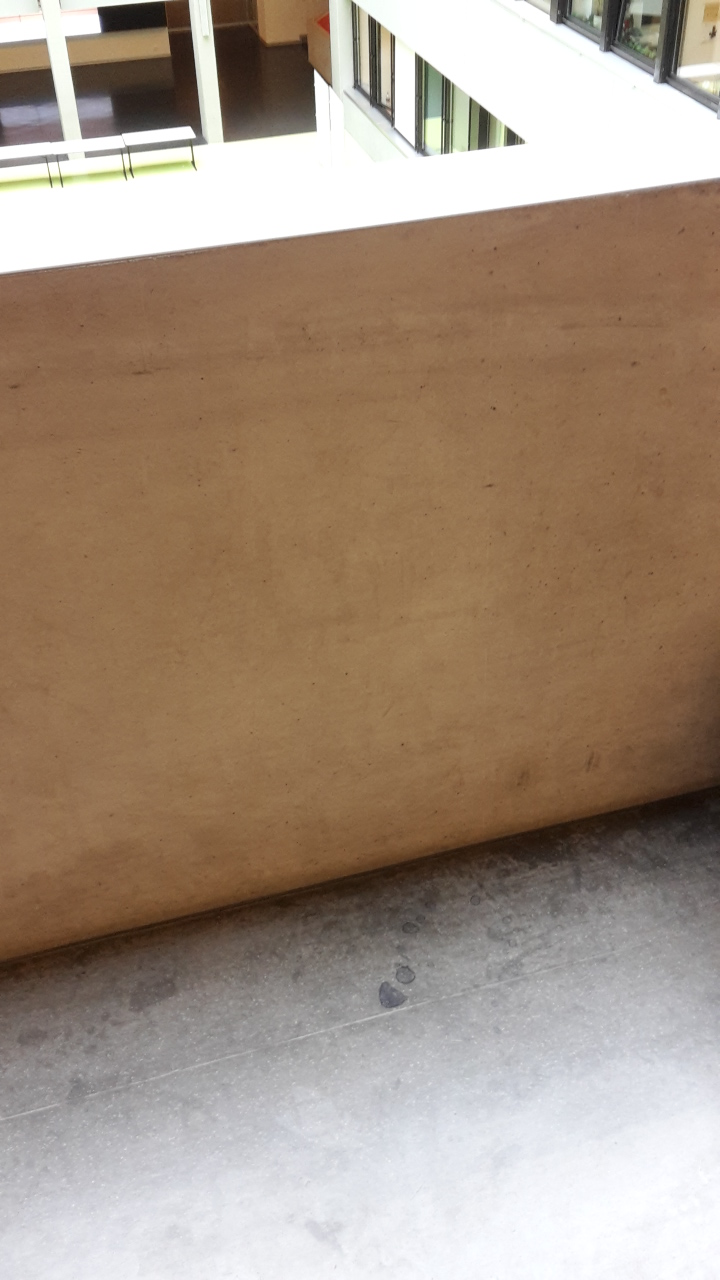
\includegraphics[width=.3\linewidth]{pictures/concrete_wall.jpg}\quad
	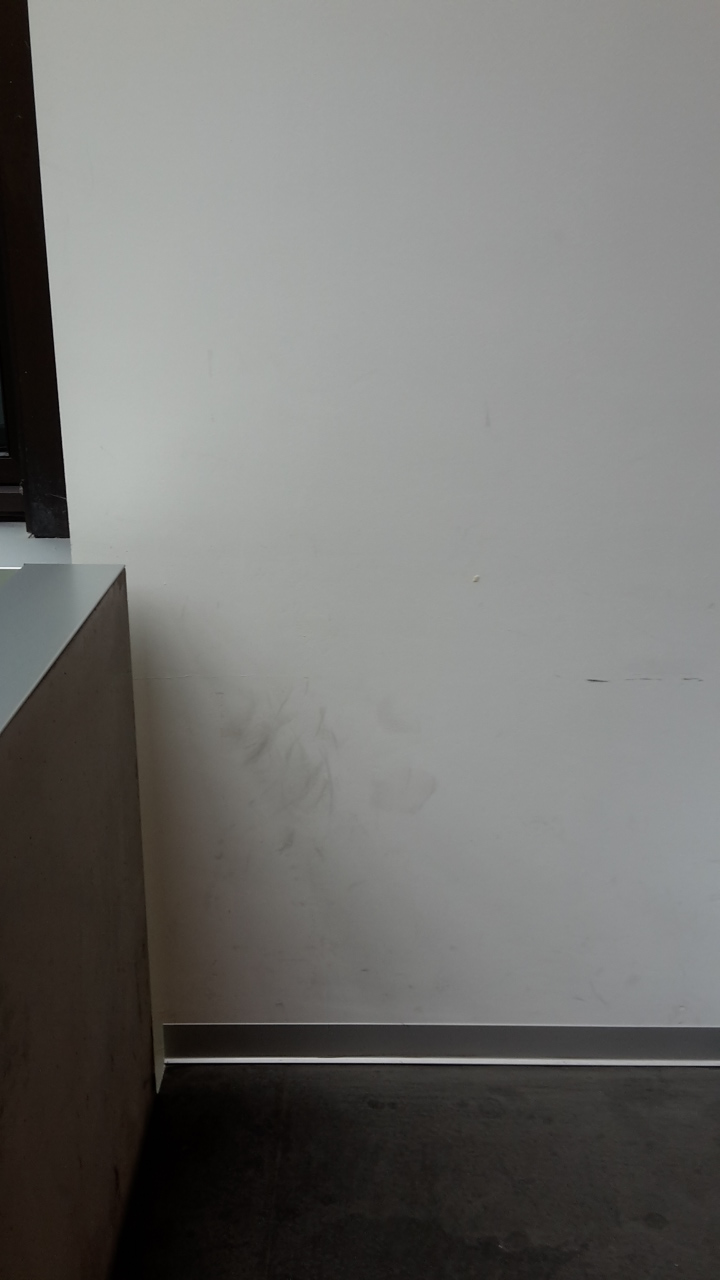
\includegraphics[width=.3\linewidth]{pictures/white_wall.jpg}\quad
	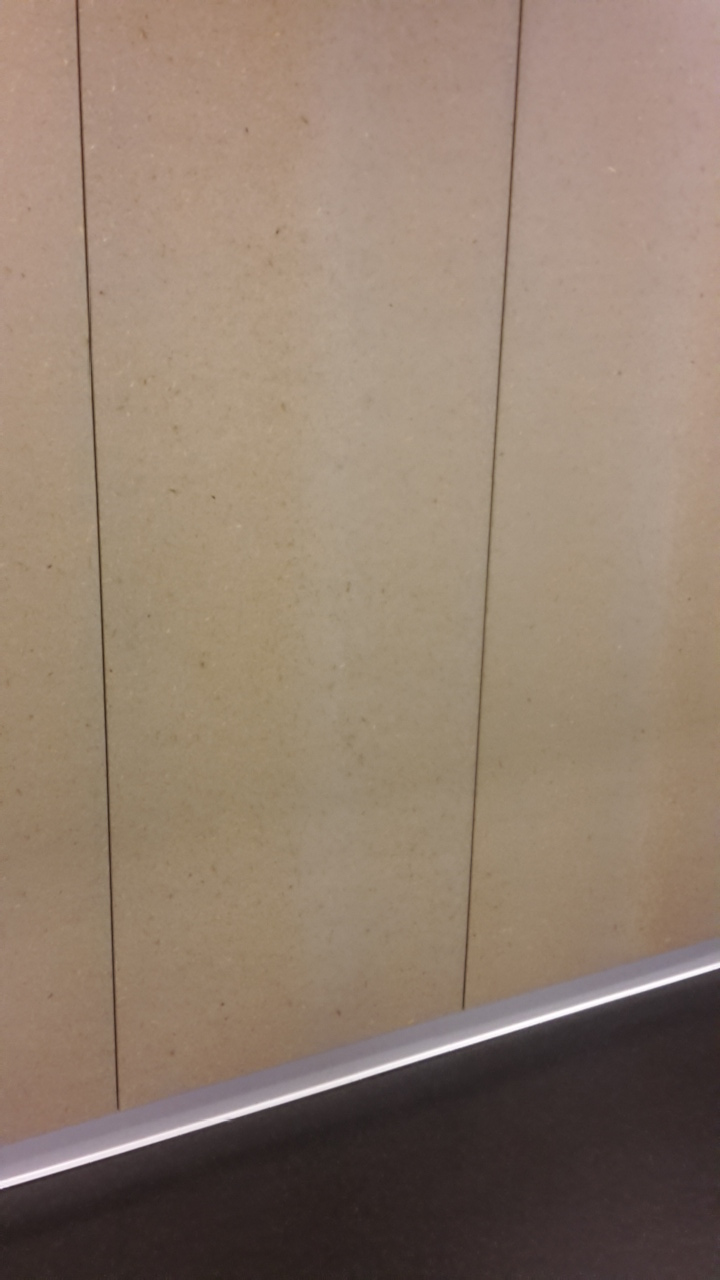
\includegraphics[width=.3\linewidth]{pictures/wooden_wall.jpg}
	\caption{Different surfaces used for the evaluation.}
	\label{fig:surfaces}
\end{figure}
\begin{figure}
	\centering
	\begin{minipage}{0.4\textwidth}
		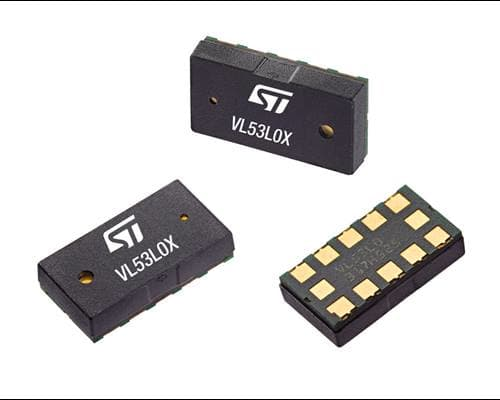
\includegraphics[width=0.9\linewidth]{pictures/vl53l0x_article2.jpg}
		\caption{\textit{VL53L0X} ranging and gesture detection sensor}
		\label{fig:sensor}
	\end{minipage}
	\quad
	\begin{minipage}{0.4\textwidth}
		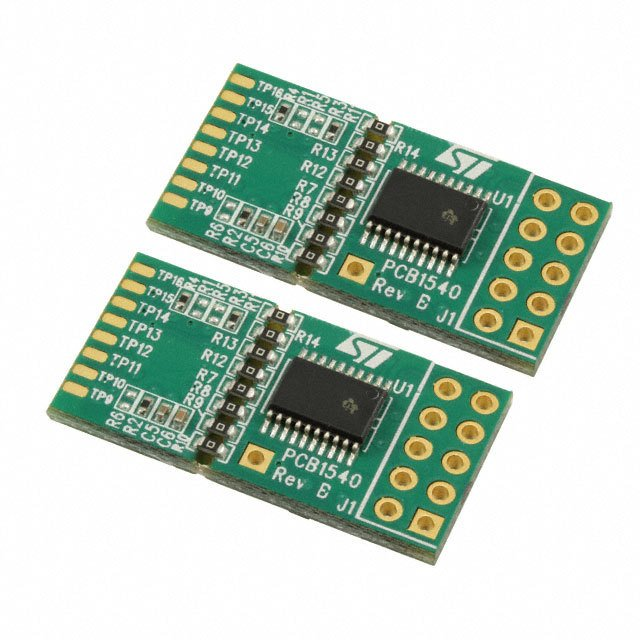
\includegraphics[width=0.9\linewidth]{pictures/53L0-SATEL-I1.jpg}
		\caption{\textit{53L0-SATEL-I1} Satellite boards based on \textit{VL53L0X} ranging and gesture detection sensor}
		\label{fig:satellite}
	\end{minipage}
\end{figure}
\begin{table}[]
	\centering
	\caption{Range profiles}
	\label{tab:profile}
	\resizebox{\textwidth}{!}{%
		\begin{tabular}{|c|c|c|c|}
			\hline
			\textbf{Range Profile} & \textbf{Range Timing Budget} & \textbf{Typical Performance} & \textbf{Typical Application}                                                             \\ 
			\specialrule{.2em}{.1em}{.1em} 
			Default Mode           & 30 ms                        & 1.2 m                        & Standard                                                                                 \\ \hline
			High Accuracy          & 200 ms                       & 1.2 m                        & Precise Measurement                                                                      \\ \hline
			Long Range             & 33 ms                        & 2 m                          & \begin{tabular}[c]{@{}c@{}}Long Rangin,\\  only for dark conditions (no IR)\end{tabular} \\ \hline
			High Speed             & 20 ms                        & 1.2 m                        & \begin{tabular}[c]{@{}c@{}}High Speed, \\ where accuracy is not important\end{tabular}   \\ \hline
		\end{tabular}%
	}
\end{table}
We evaluated the sensor's performance using different target surfaces and at different lightning conditions. During the measurements we varied the angle and distance relative to the target. For the ground truth measurement we used a yardstick and a protractor. We conducted 100 measurements for every measurement setup. The surfaces used for the evaluation were a white plastered wall, a concrete wall and a wooden wall (\cref{fig:surfaces}).\\
The sensor uses IR for the measurement. Another strong IR source in the proximity of the sensor, e.g., the sun, reduces the accuracy and might even obstruct the sensor from making a measurement. To get reliable data, first, we filtered out the failed measurements, i.e., removing all data points with a value greater than 8000, and, second, rejected outliers with Mahalonobis distance and filtered the remaining data points with a Kalman filter (\cref{alg:filter}). For the filter we assumed constant distance in the process model:
\begin{equation}
\label{eq:filter}
\begin{split} 
x_k & = x_{k-1} \\
y_k & = x_k + v_k \text{ ,}
\end{split}
\end{equation}
where $x_k$ is the distance. The noise process $v_k$ is white, zero-mean, uncorrelated, and has a known covariance matrix  $R_k$.\\
The assumption of constant distance is only valid for the evaluation of the sensor. In case of a moving sensor or target, a dynamic process model has to be developed. Further, a IMU should be used for the a priori state estimate.\\
\begin{algorithm}
	\caption{Filter}\label{alg:filter}
	\begin{algorithmic}[1]
		\Procedure{FILTER}{ }
		\State $y_{data}\gets \text{raw data points}$ 
		\State Filter out corrupted data points from $y_{data}$ \\
		\textit{Initzialization:}
		\State $\hat{x}^+_0\gets\text{initial measurement }y_{data}(0)$
		\State $R_k\gets\unit[27^2]{mm^2}$ \Comment{variance of the measurements}
		\State $P^+_0\gets \unit[30]{mm^2}$ \Comment{got this value from tuning}
		\For{ each $k = (0, \text{ number of data point]}$}	
		\State  $P^-_k \gets \text{Covariance of estimation error}$
		\State	$K_k \gets \text{Kalman gains}$
		\EndFor \\
		\textit{State Estimation:}	 
		\For{ each $k = (0, \text{ number of data point]}$}
		\State \Call{Mahal}{$y_{data,k}$} \Comment{Outliers rejection with mahalanobis distance}
		\State $\hat{x}^-_k \gets \text{a priori state estimate}$
		\State $\hat{x}^+_k \gets \text{a posteriori state estimate}$
		\EndFor
		\State \Return $\hat{x}^+_k$
		\EndProcedure
		
	\end{algorithmic}
\end{algorithm}


\section{Pixhawk}
\label{sec:pixhawk}
We use a \textit{pixhawk mRo} as a autopilot which has the benefit of being versatile. Thus, our avoidance system is not only appliable to the platform we have used for testing, but moreover the avoidance system can be applied to all platforms using a pixhawk autopilot.\\
To couple the VL53L0X sensors with the pixhawk we first tried to connect four different VL53L0X sensors to the pixhawk via I2C bus. Compiling the firmware on the pixhawk resulted in a flash overflow due to the large sensor API. The API is essential for the initialization and calibration of the VL53L0X sensors. To circumvent this problem, we connect the four sensors to the previously used mbed LPC1768 microcontroller and send the data from the mbed microcontroller to the pixhawk via I2C. Therewith, we can compile the API on the mbed microcontroller and we just have to read the data on the pixhawk. The repulsive force of a target is then computed on the pixhawk using a potential field.


\section{Potential Field}
\label{sec:potential field}
The basic idea behind all potential field approaches is that the robot is attracted towards a goal, while being repelled by an obstacle. For our system, we are only interested in the repulsive potential $U_{rep}$. This potential should be very strong when the system is close to a obstacle and on the same time the system should not be influenced by obstacles far away. One example of such a repulsive field is:
\begin{equation}
\label{eq:pot field}
\centering
U_{rep}(q)=\begin{cases}
\dfrac{1}{2}k_{rep}\left(\dfrac{1}{\rho (q)}-\dfrac{1}{\rho_0}\right)^2 & \text{if } \rho(q)\leq\rho_0 \\
0 & \text{if } \rho(q)>\rho_0 \text{ ,}
\end{cases}
\end{equation}
where $k_{rep}$ is a scaling factor, $\rho(q)$ is the minimal distance from the obstacle to the system position $q$, and $\rho_0$ is the distance of influence of the object. The repulsive potential function is positive or zero and tends to infinity as $q$ gets closer to the object.\\
If the object boundary is convex and piecewise differentiable, $\rho(q)$ is differentiable everywhere in the free configuration space. This leads to the repulsive force $F_{rep}$:
\begin{equation}
\label{eq:force}
\begin{split}
F_{rep} &=-\Delta U_{rep}(q)\\
&=	\begin{cases}
k_{rep}\left(\dfrac{1}{\rho(q)}-\dfrac{1}{\rho_0}\right)\dfrac{1}{\rho^2(q)}\dfrac{q-q_{obstacle}}{\rho(q)} & \text{if }\rho(q)\leq\rho_0\\
0 & \text{if }\rho(q)\geq\rho_0
\end{cases}
\end{split}
\end{equation}
This repulsive force has now to be converted into corrective attitude angles with a further factor $k_{att}$. This yields: 
\begin{equation}
	\label{eq:angles}
	\Omega_{corr} =\begin{pmatrix}
	\theta_{corr} \\ \phi_{corr} \\ \psi_{corr}
	\end{pmatrix} = k_{att}\cdot F_{rep} \text{ ,}
\end{equation}
where $\theta_{corr} \text{, } \phi_{corr} \text{ and } \psi_{corr}$ are the corrective pitch, roll and yaw angles, respectively. In our approach, two ranging sensors measure the distance to an obstacle in x-direction  ($d_{+x}$ \& $d_{-x}$) and two sensors measure the distance to an obstacle in y-direction ($d_{+y}$ \& $d_{-y}$). The idea is that $d_{+x}$ and $d_{-x}$ are used to compute the corrective pitch $\theta_{corr}$ and $d_{+y}$ and $d_{-y}$ are used to compute the corrective roll $\phi_{corr}$. The corrective roll $\psi_{corr}$ is set to zero:
\begin{equation}
	\label{eq:angle sp}
	\Omega_{corr} =
	\begin{pmatrix}
	\theta_{corr} \\ \phi_{corr} \\ \psi_{corr}
	\end{pmatrix} =
	k_{corr}\cdot 
	\begin{pmatrix}
	\left(\dfrac{1}{d_{-x}}-\dfrac{1}{\rho_0}\right)\dfrac{1}{d_{-x}^2}-\left(\dfrac{1}{d_{+x}}-\dfrac{1}{\rho_0}\right)\dfrac{1}{d_{+x}^2}\\\\
	\left(\dfrac{1}{d_{-y}}-\dfrac{1}{\rho_0}\right)\dfrac{1}{d_{-y}^2}-\left(\dfrac{1}{d_{+y}}-\dfrac{1}{\rho_0}\right)\dfrac{1}{d_{+y}^2} \\\\
	0
	\end{pmatrix}
	\text{ ,}
\end{equation}

where $k_{corr}=k_{att}\cdot k_{rep}$. These corrective angles (\cref{eq:angle sp}) are directly sent to the attitude controller and added to the current attitude set-points $\Omega_{sp}$

\begin{equation}
\label{eq:new sp}
	\Omega_{sp}' = \Omega_{sp} + \Omega_{corr} \text{ ,}
\end{equation}
where $\Omega_{sp}'$ are the new set-point. \\
To validate \cref{eq:angle sp} we have used Matlab. We have included an upper threshold for the corrective angle (\cref{fig:pf matlab}). The potential field behaves as desired. The corrective angle increases exponentially with a smaller distance to the wall. 

\begin{figure}
	\centering
	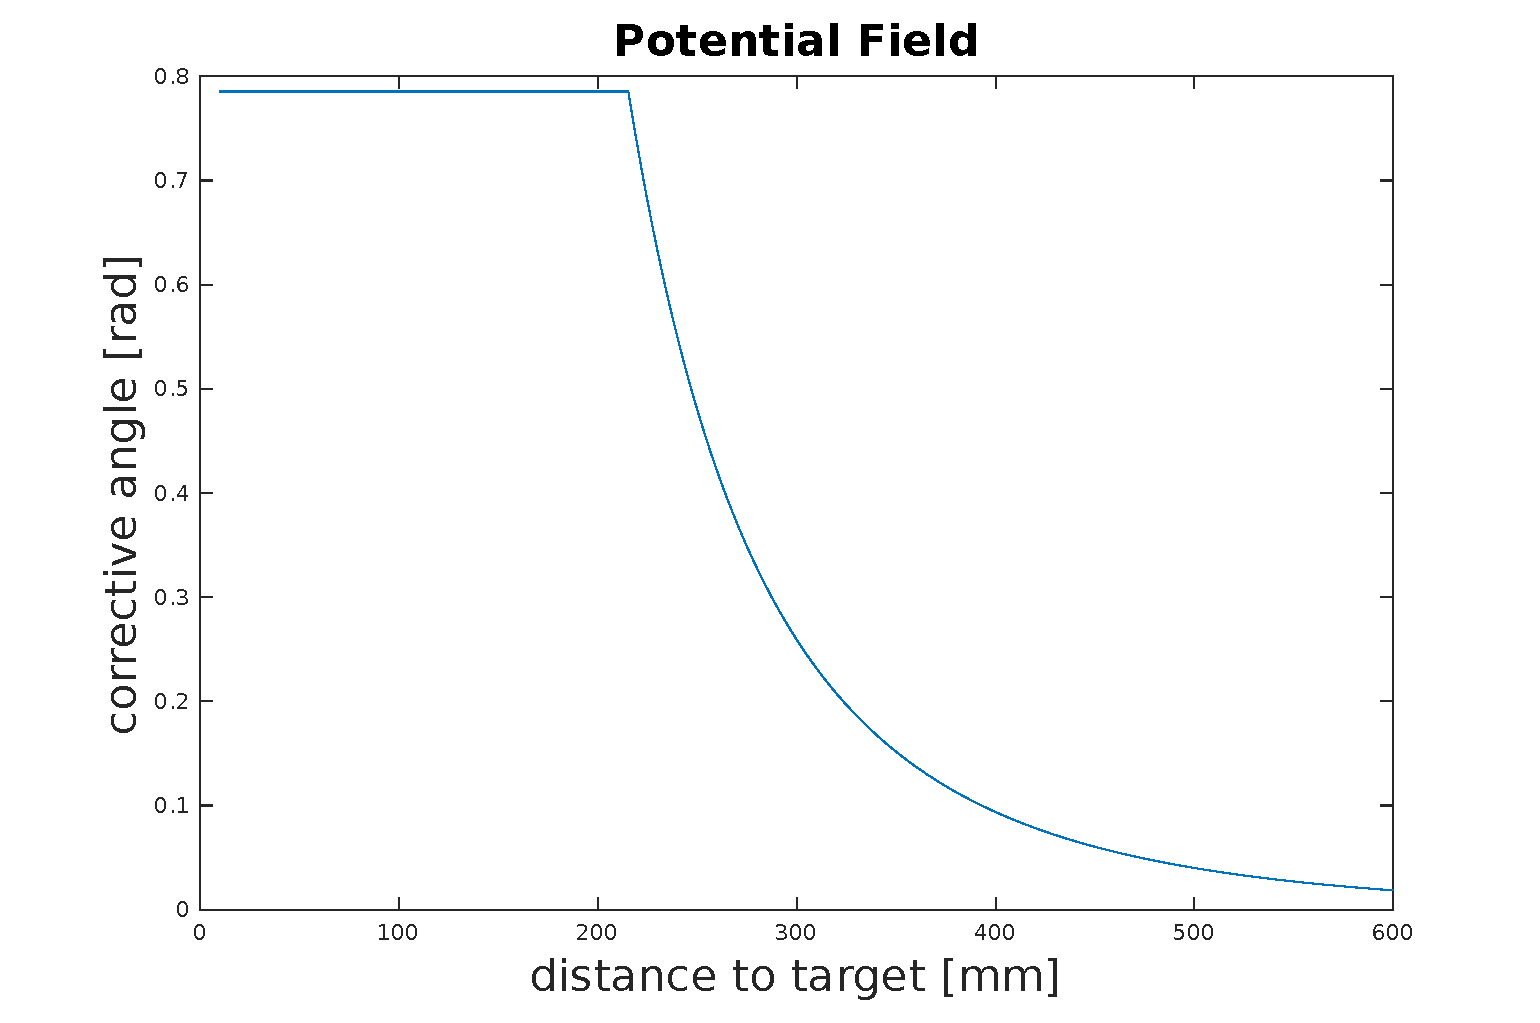
\includegraphics[width=0.8\linewidth]{pictures/plot_pf_matlab.pdf}
	\caption{Plotted \cref{eq:angle sp}. $k_{corr}=10000000$, $\theta_{threshold}=0.25\pi$ and $\rho_0=\unit[1000]{mm}$. As the distance decreases the corrective angle increases exponentially. At around \unit[200]{mm} the upper threshold $\theta_{threshold}$ is reached}
	\label{fig:pf matlab}
\end{figure}


\section{Testing}
\label{sec:testing}
For the testing of the whole avoidance system we have used a quadrocopter platform based on the DJI 450 Flame Wheel frame (\cref{fig:loon}). To validate the performance of the implemented potential field we detached the propellers, approached a wall while holding the platform by hand and observed how the motors responded while simultaneously logging the data. Next, we mounted the propellers and again approached a wall holding the platform by hand. Last, we piloted the platform with a remote control towards the wall and logged the potential field behaviour. For the parameters we set for the gain $k_{corr}=800000000$, for the distance of influence $\rho_0=\unit[1500]{mm}$ and for the corrective angle threshold $\Omega_{corr,thresh}=\unit[\pm1.5]{rad}$.
\begin{figure}
	\centering
	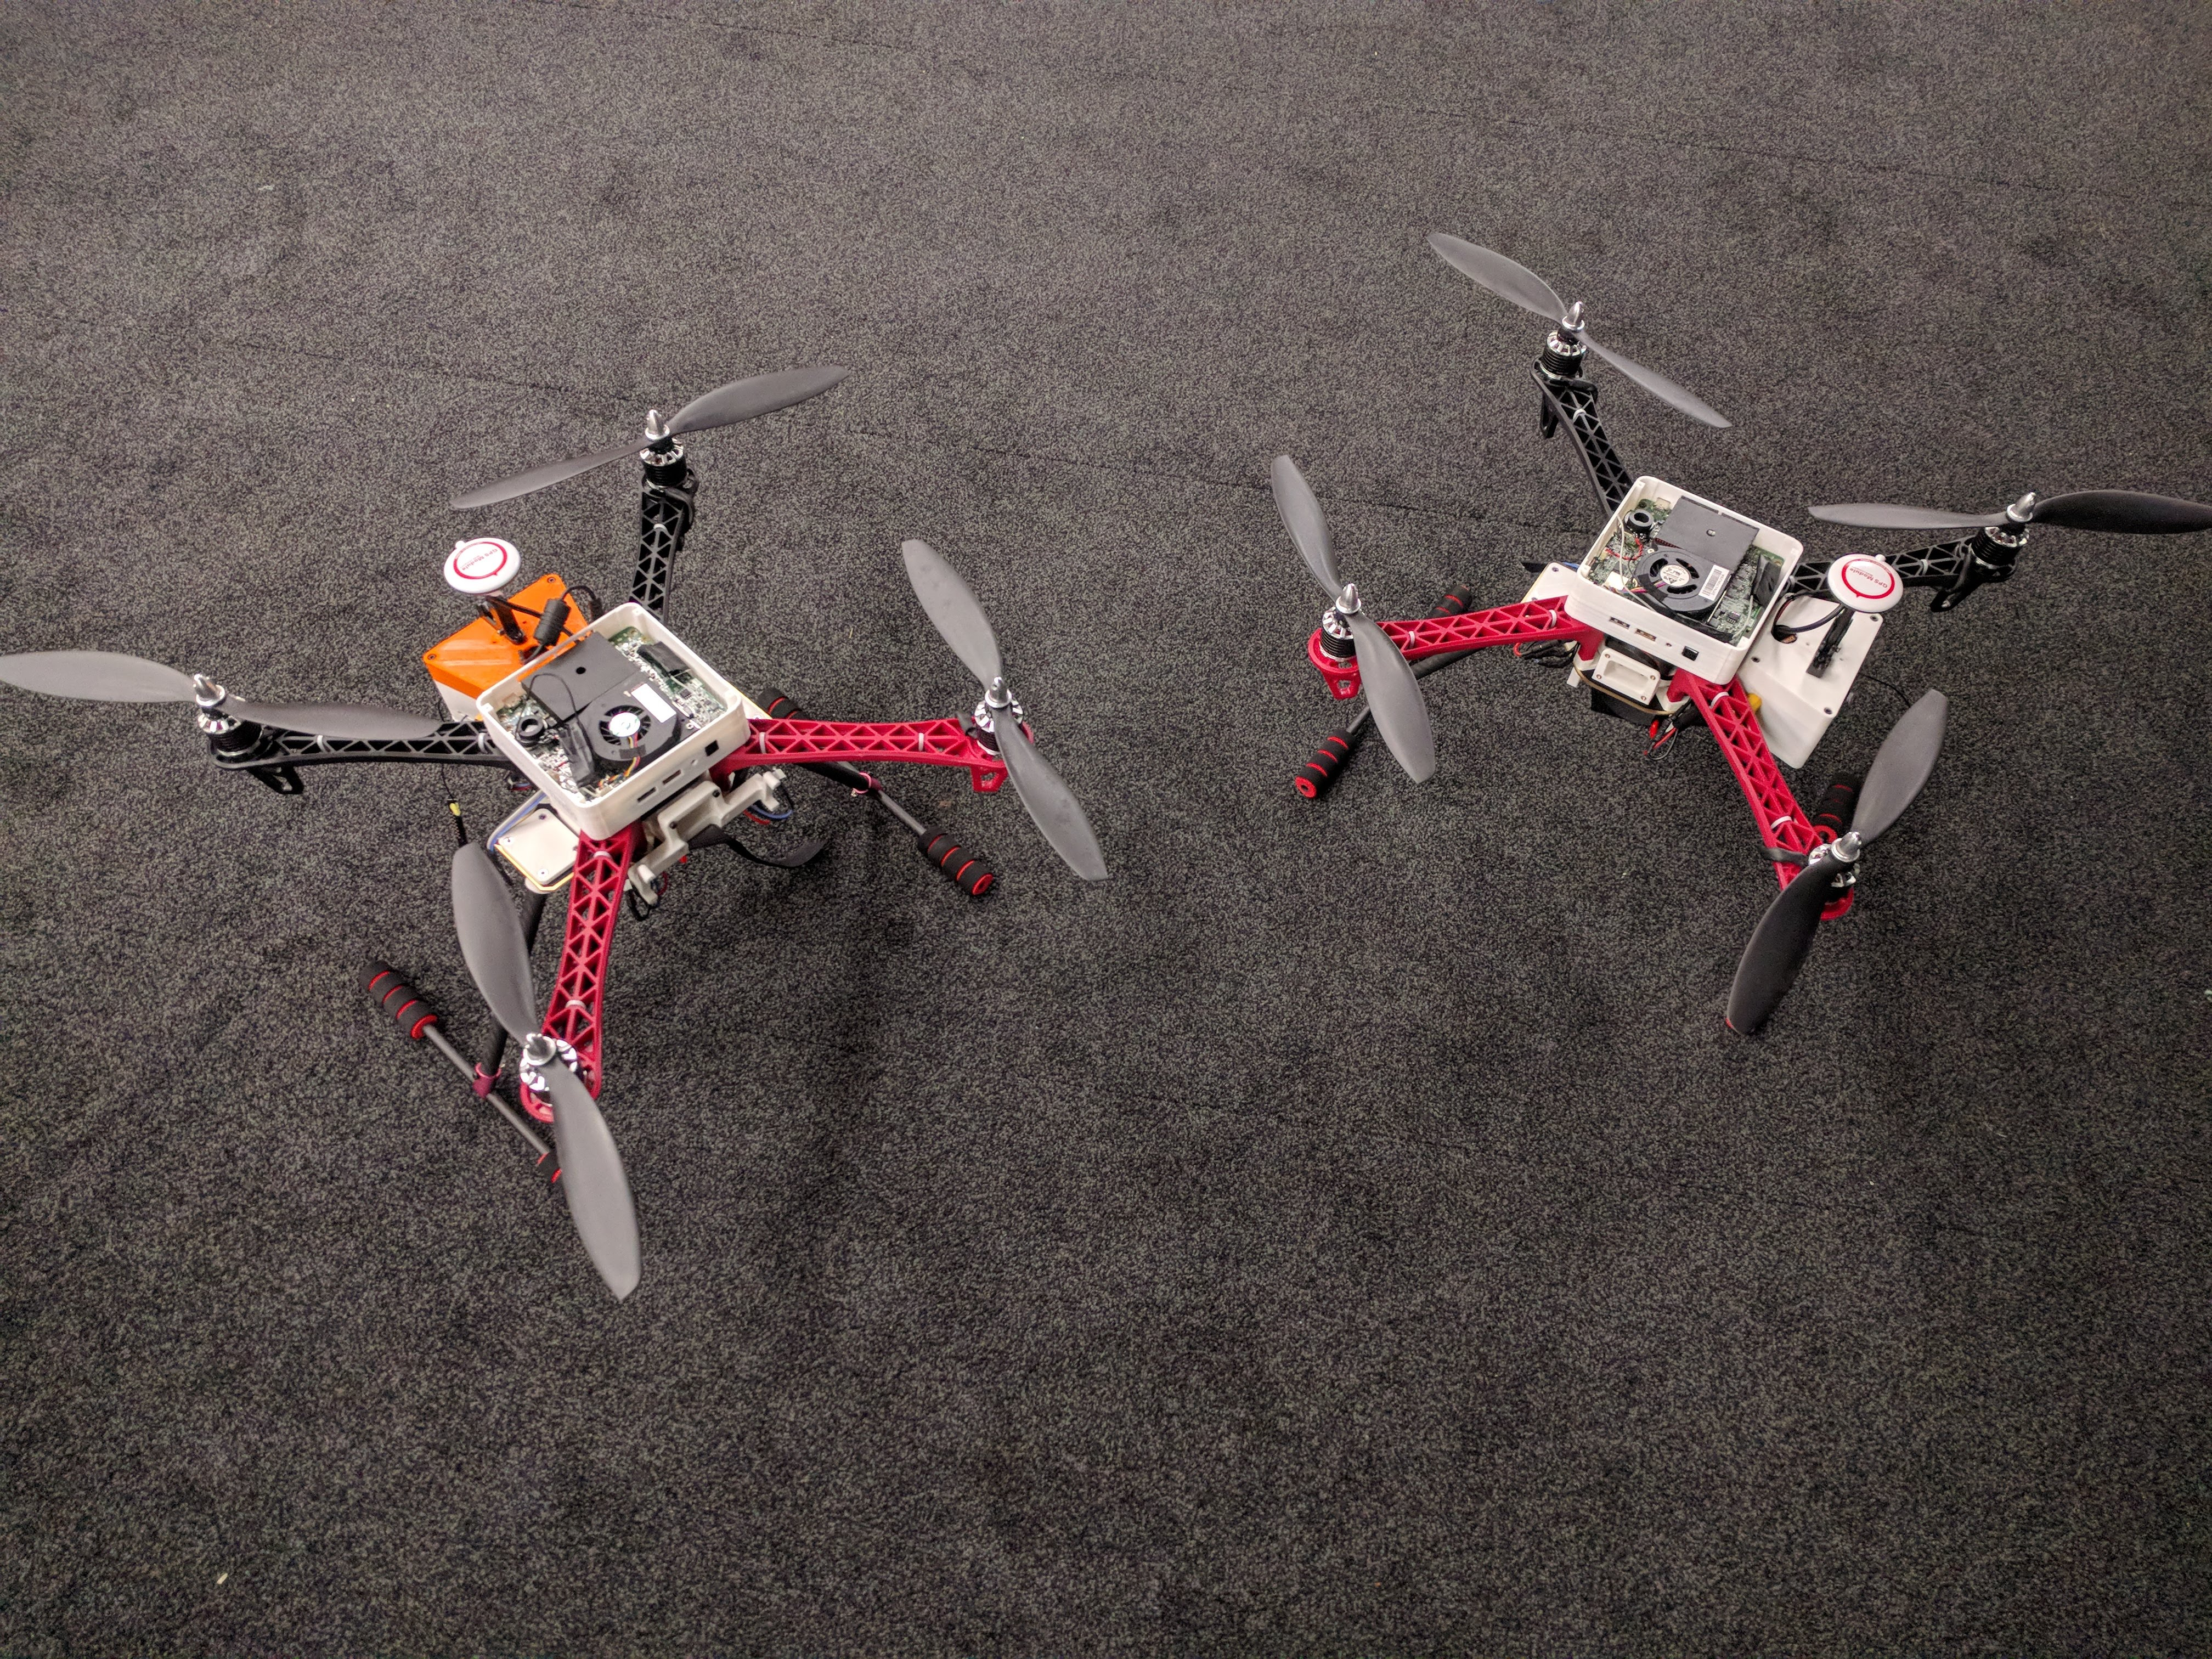
\includegraphics[width=0.62\linewidth]{pictures/loons.jpg}
	\caption{Platform used for testing based on the DJI 450 Flame Wheel.}
	\label{fig:loon}
\end{figure}